\documentclass{article}
\usepackage[utf8]{inputenc}
\usepackage{graphicx}
\graphicspath{ {images/} }
\usepackage{listings}
\usepackage{color}
\usepackage{textcomp}
\usepackage{multicol}
\usepackage{float}

\title{CMPE460 Project 2 Report}
\author{
  Yiğit Özkavcı \\
  \texttt{2013400111} \\
  \texttt{yigit.ozkavci@boun.edu.tr}
}
\date{February 2018}

\begin{document}

\maketitle

\tableofcontents

\section{Introduction}

In this project, we've improved the work done in the previous project: ray tracer. We will describe the improvements done and features developed with respect to the old version of our solution.

In section \ref{phong}, we illustrate how we've implemented Phong Illumination Model in our renderer. In section \ref{multiple-ls}, we talk about multiple light sources and we show different examples with multiple light sources in different positions. Lastly, in section \ref{ground}, we will show how a single ground plane is represented and how do we observe shadow of the spheres on this ground plane.

\newpage

\section{Phong Illumination Model}
\label{phong}

Phong Illumination Model requires us to consider normal vectors of the intersections while we are "illuminating" a pixel. Let's dig into what illumination means in our project's context: when first shooting the rays, we capture the intersections with a color multiplier of AMBIENT\_COLOR. If AMBIENT\_COLOR is zero, we initially observe a black shape. Then, after we shoot this ray, we immediately try to illuminate this point. To illuminate, we traverse the light sources, and see if there is an obsticle on our way to light source, if there is, we discard it. If we can reach to a light source from our intersection, this means light source should illuminate our point.

This was already done in the previous project, and in order to apply Phong Illumination Model, we considered the angle between our ray vector to the light source and the normal vector of the object (sphere or plane in this project) at the intersection point. This angle determines how "powerful" should the illumination be.

Note: for all examples, we have two spheres:


\subsection{Examples}
\begin{centering}
\begin{figure}[H]
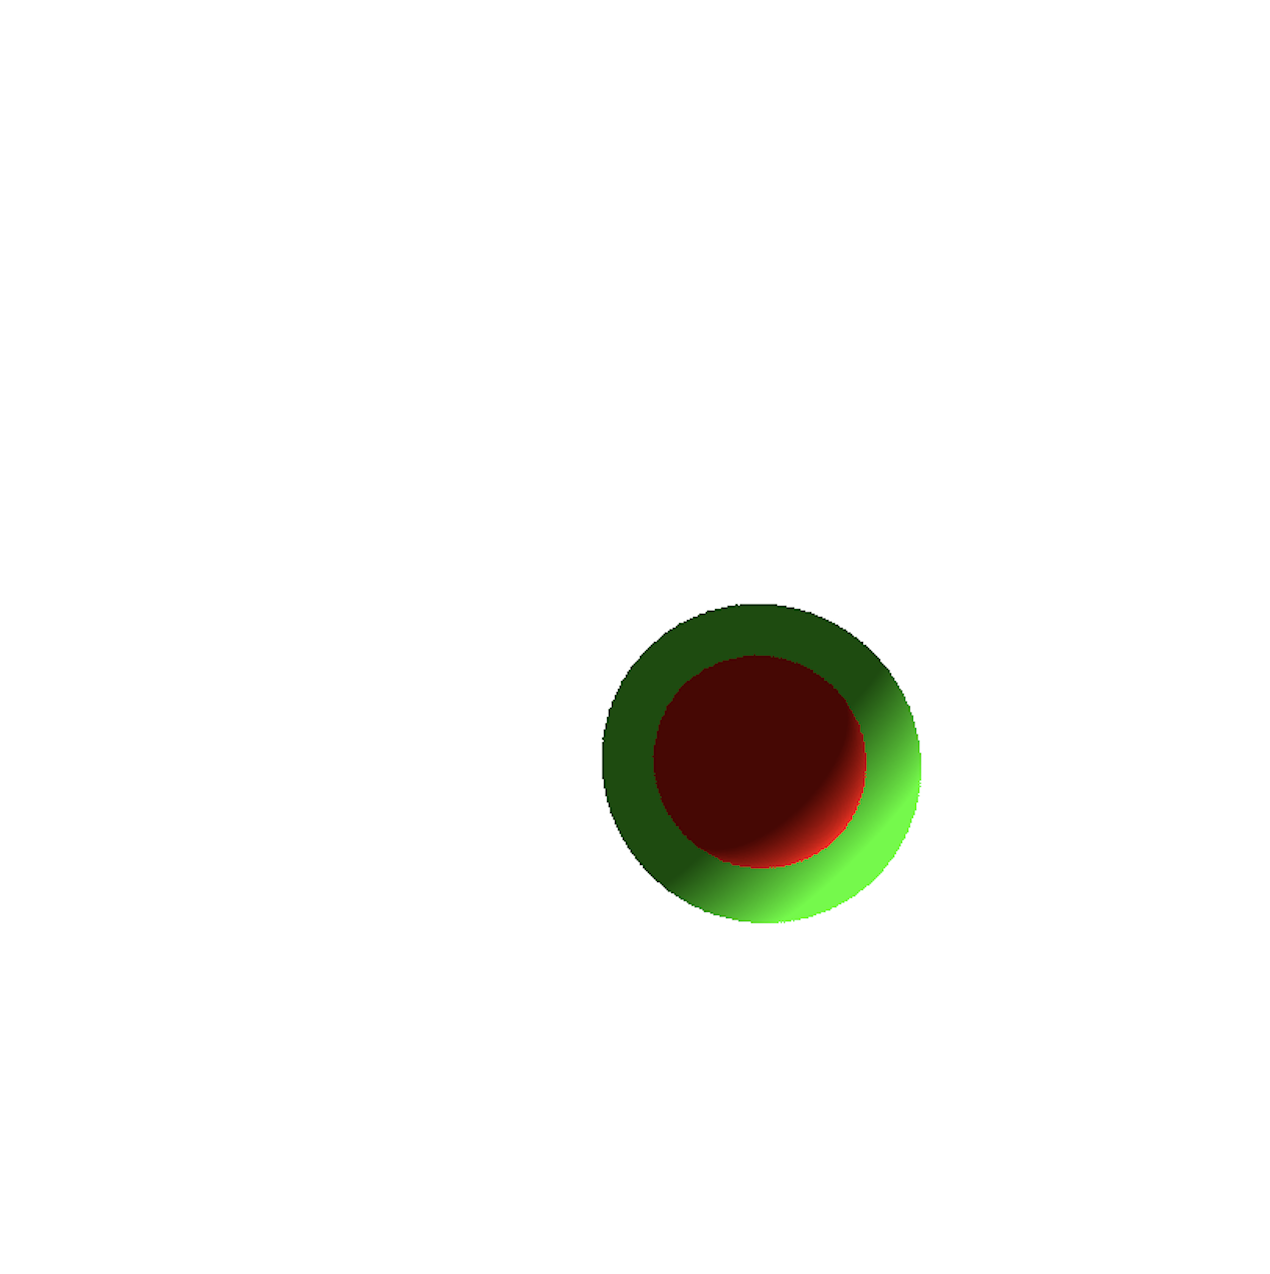
\includegraphics[width=1\textwidth]{./images/phong.png}
\caption{Phong Illumination}
\label{fig:phong}
\end{figure}
\end{centering}

\newpage

\section{Multiple Light Sources}
\label{multiple-ls}
Introducing multiple light sources was almost trivial for this project since we already had the business logic for illuminating points. There was no bugs caused by this multiple light source approach.

\subsection{Examples}
\begin{centering}
\begin{figure}[H]
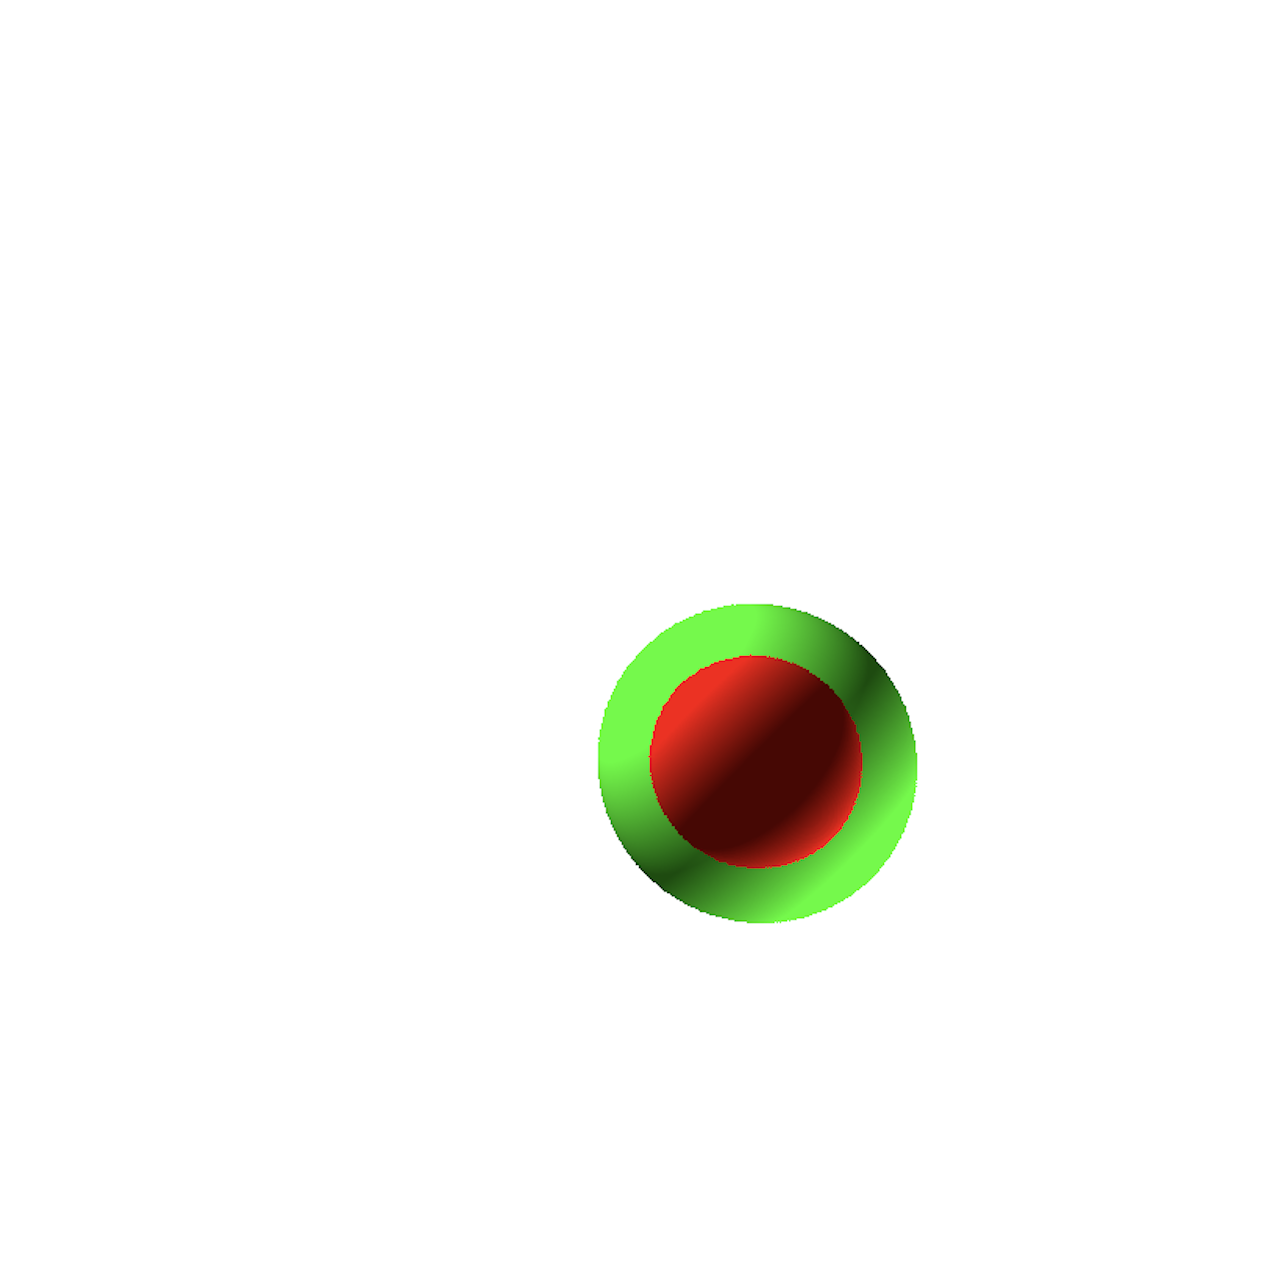
\includegraphics[width=1\textwidth]{./images/multiple-ls.png}
\caption{Multiple Light Sources at (500, 500, 500) and (-500, -500, 500) }
\label{fig:ml1}
\end{figure}
\begin{figure}[H]
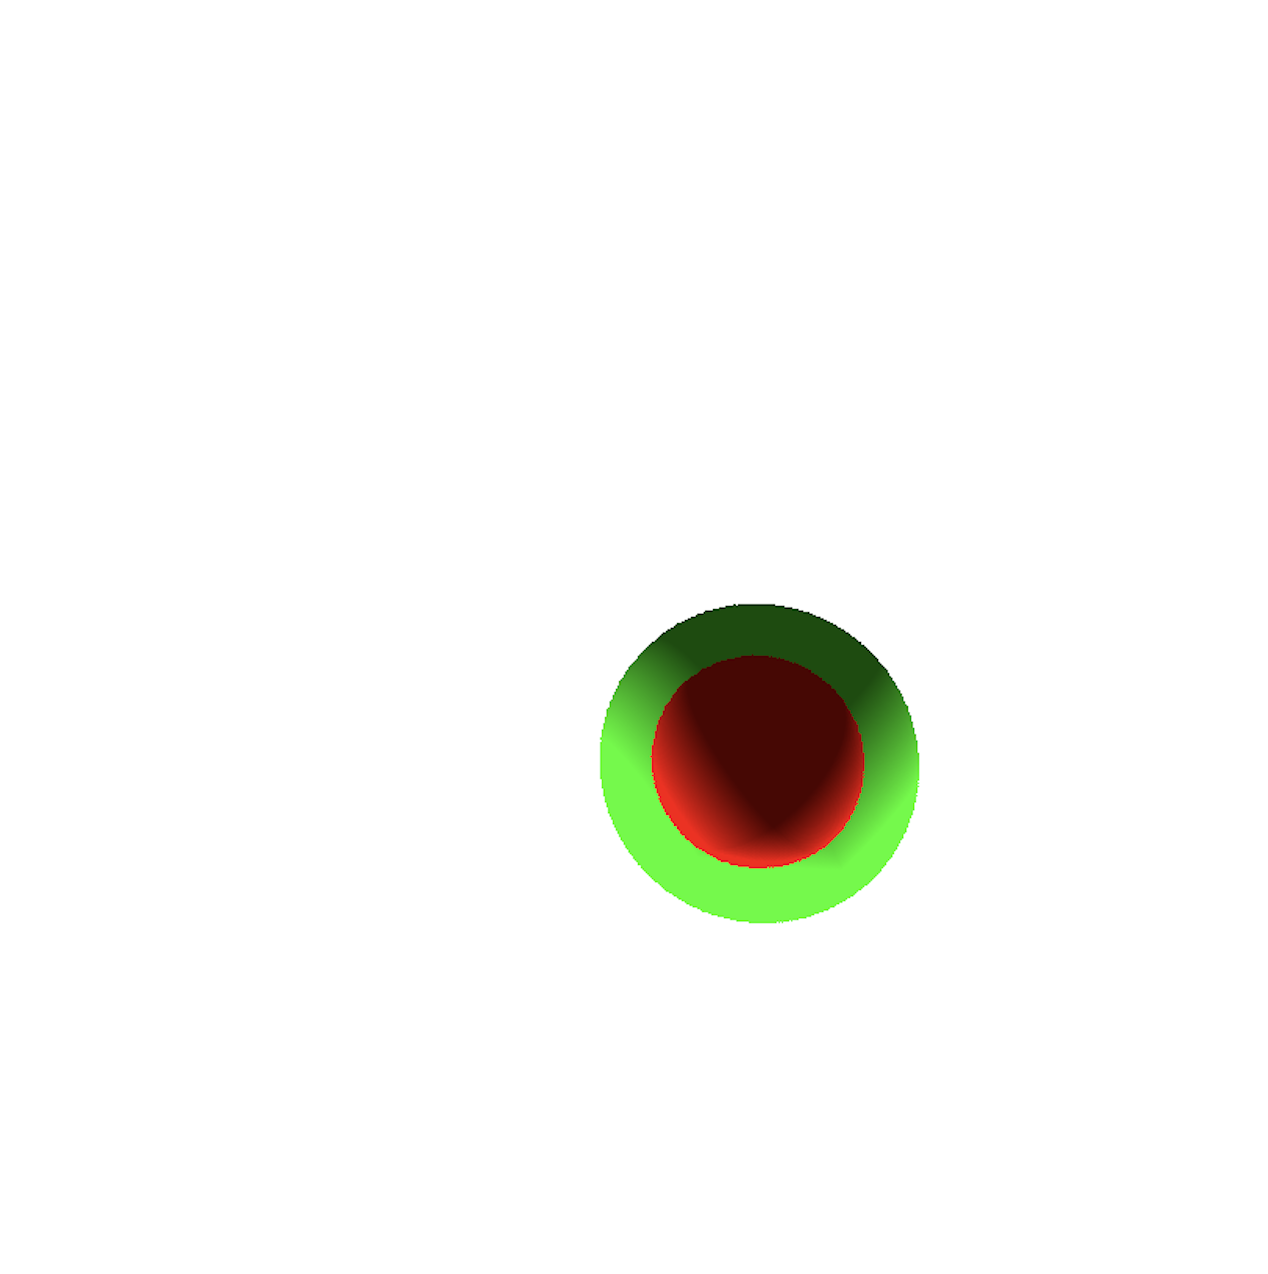
\includegraphics[width=1\textwidth]{./images/multiple-ls2.png}
\caption{Multiple Light Sources at (500, 500, 500) and (-500, 500, 500) }
\label{fig:ml2}
\end{figure}
\end{centering}

\newpage

\section{Ground Plane}
\label{ground}

Adding a ground plane was probably the hardest task in this project. It introduced many bugs. After a ground plane is recognised as a shape in our codebase, we needed to generalize some of the concepts, since most of the time we assumed we would only work with sphere objects.

\subsection{Examples}
\label{examples}

\begin{centering}
\begin{figure}[H]
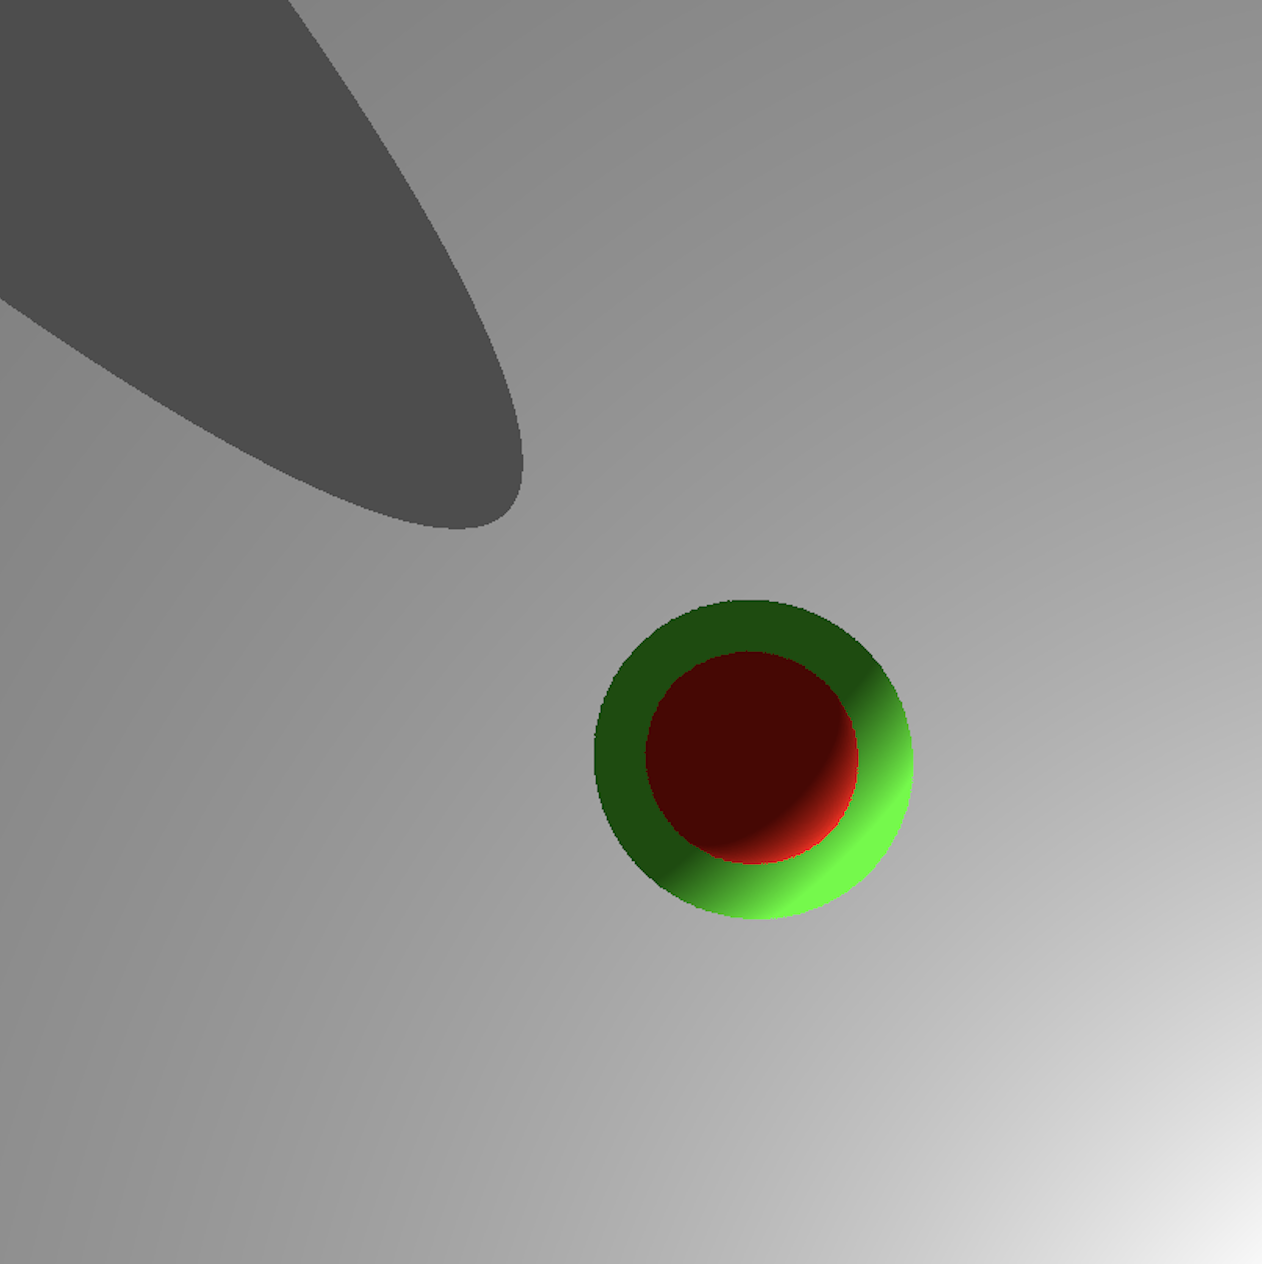
\includegraphics[width=1\textwidth]{./images/white-bg-ambient-03.png}
\caption{White Ground Plane with Ambient Light Coefficient of 0.3}
\label{fig:gp1}
\end{figure}
\begin{figure}[H]
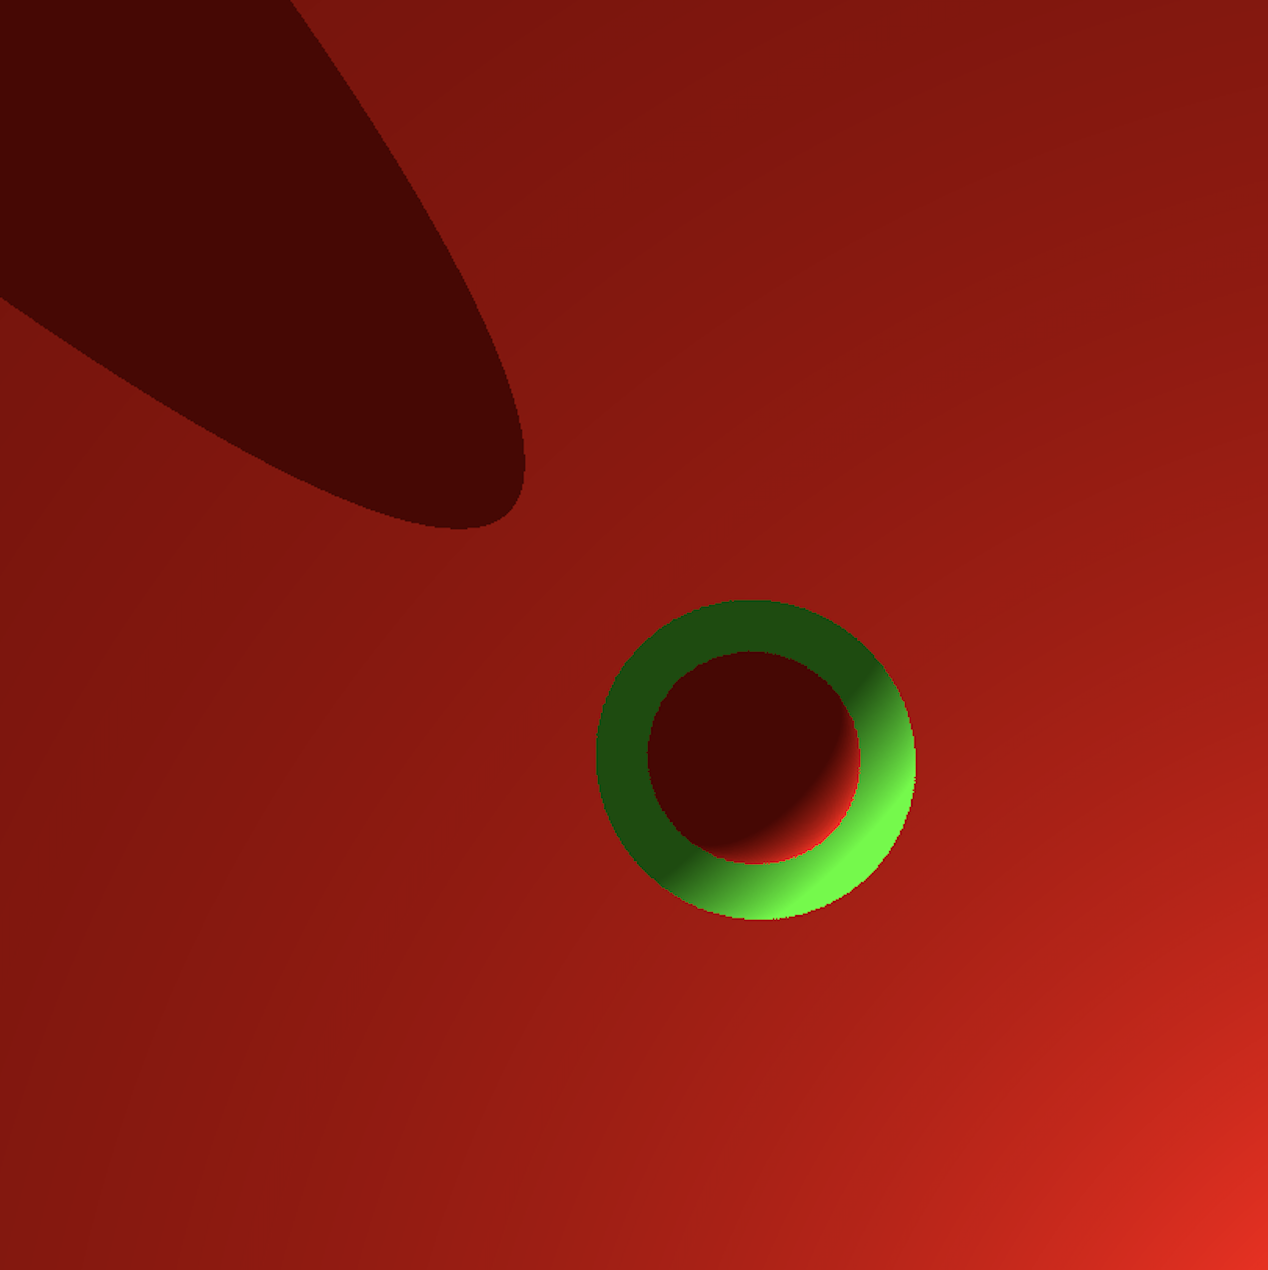
\includegraphics[width=1\textwidth]{./images/red-bg-ambient-03.png}
\caption{Red Ground Plane with Ambient Light Coefficient of 0.3}
\label{fig:gp2}
\end{figure}
\begin{figure}[H]

\includegraphics[width=1\textwidth]{./images/red-bg-ambient-05.png}
\caption{Red Ground Plane with Ambient Light Coefficient of 0.5}
\label{fig:gp3}
\end{figure}
\end{centering}

\end{document}
